\documentclass[11pt]{article}
\usepackage{natbib,mybigpackage}
\usepackage{algorithm}
%\usepackage{program}
%\usepackage{algpseudocode}
\usepackage{algorithmic}
\usepackage{listings}


\def\xbf{\mathbf{x}}
\def\zbf{\mathbf{z}}
\def\xibf{\mathbf{\xi}}
\title{MA 226 - Assignment Report 6}
\author{Ayush Sharma\\150123046}
\begin{document}
\titlepage
\newpage

\begin{enumerate}
\item[Q 1] Use the Box-Muller method and Marsaglia-Bray method to do the following :\\
(a) Generate a sample of 100, 500 and 10000 values from $\mathcal{N}(0, 1)$. Hence find the sample mean and variance.\\
(b) Draw histogram in all cases.

\item[Q 2] Now use the above generated values to generated samples from $\mathcal{N}(\mu = 0, \sigma^2 = 5)$ and $\mathcal{N}(\mu = 5, \sigma^2 = 5)$.
Hence plot the empirical (from sample with size 500) distribution function and theoretical distribution function in the same plot.\\
(Use R / you should also try making the step function in C).

\item[Q 3] Keep a track of the computational time required for both the methods. Which method is faster ?

\item[Q 4] For the Marsaglia-Bray method keep track of the proportional of values rejected.
How does it compare with $1-\frac{\pi}{4}$ ?
\end{enumerate}
\newpage
\noindent{\textbf{Solution}:}

\noindent{}Generating random number from the standard normal distribution by the \textbf{Box-Muller} method :\\
This algorithm generates a sample from a bivariate standard normal, each component of which is thus a univariate standard normal.\\
The algorithm is based on the following two properties of bivariate normal. If $Z$ is $N(0, 1)$, then
\begin{itemize}
	\item $R = Z_{1}^{2} + Z_{2}^{2}$ is exponentially distributed with mean 2, i.e., $P(R \leq x) = (1 - e^{-\frac{x}{2}})$.
	\item Given $R$, the point $(Z_1, Z_2)$ is uniformly distributed on the circle of radius $\sqrt{R}$ centered at the origin.
\end{itemize}
Thus to generate $(Z_1, Z_2)$ we first generate $R$ and then choose a point uniformly from the circle of radius $\sqrt{R}$.
To sample from the exponential distribution we may set $R = −2\log{U_1}$ with $U_1 \sim \mathcal{U}(0,1)$.\\
To generate a random point on a circle we may generate angle uniformly between 0 and $2\pi$ and map the angle to a point on the circle.
The random angle may be generated as $V = 2\pi U_2$ with $U_2 \sim \mathcal{U}(0,1)$.\\
The corresponding point on the circle has co-ordinate $(\sqrt{R}\cos{V}, \sqrt{R}\sin{V})$.\\
The complete algorithm is :
\begin{algorithm}[H]
\caption{Generating Random number from the standard normal distribution by the Box-Muller method}
\begin{algorithmic}[1]
\STATE Generate $U_1, U_2$ from $\mathcal{U}(0,1)$.
\STATE Generate $R$ and $V$ from the relations $R = −2\log{U_1}$ and $V = 2\pi U_2$.
\STATE Generate $Z_1$ and $Z_2$ from the relations $Z_1 = \sqrt{R}\cos{V}$ and $Z_2 = \sqrt{R}\sin{V}$.
\STATE Return $Z_1$ and $Z_2$.
\end{algorithmic}
\end{algorithm}

\noindent{}Generating random number from the standard normal distribution by the \textbf{Marsaglia and Bray} method :\\
Marsaglia and Bray developed a modification of the Box-Muller method that reduces computing time by avoiding evaluation of the cos and sin functions.
The Marsaglia-Bray method instead uses acceptance-rejection method to sample paths uniformly in the unit disc and transforms the points to normal variates.\\
The transform $U_i \rightarrow 2U_i - 1$, $i = 1 : 2$ makes $(U_1, U_2)$ uniformly distributed on the square $[−1, 1] × [−1, 1]$.\\
Accepting only those pairs for which $X = U_{1}^{2} + U_{2}^{2}$ is less than or equal to 1 produces points uniformly distributed over the disc of radius 1 centered at the origin.\\
Conditional on acceptance, X is uniformly distributed between 0 and 1 so that $\log(X)$ has the same effect as $\log(U_1)$ for Box-Muller.\\
Dividing each accepted $U_1$ and $U_2$ by $\sqrt{X}$ projects it from the unit circle, on which it is uniformly distributed.\\
The algorithm is as follows :
\begin{algorithm}[H]
\caption{Generating Random number from the standard normal distribution by the Marsaglia and Bray method}
\begin{algorithmic}[1]
\STATE Generate $U_1, U_2$ from $\mathcal{U}(0,1)$.
\STATE Transform $U_1$ and $U_2$ using the relation $U_i \rightarrow 2U_i-1$,\hspace{4mm} $i = 1 : 2$.
\IF{$X \leq 1$}
	\STATE Generate $Y$ from the relation $Y = \sqrt{\frac{-2\log{X}}{X}}$.
	\STATE Generate $Z_1$ and $Z_2$ from the relation $Z_{i} = U_{i}Y$,\hspace{4mm} $i = 1 : 2$.
	\STATE Return $Z_1$ and $Z_2$.
\ELSE
	\STATE return to step 1.
\ENDIF
\end{algorithmic}
\end{algorithm}
\newpage
\noindent{Code for R}
\begin{lstlisting}
genNormal_Box_Muller<-function(sample) {
	N<-vector(length = sample);
	set.seed(1);
	for (i in seq(1, sample, 2)) {
	u<-runif(2, 0, 1);
	R = -2 * log(u[1]);
	V = 2 * pi * u[2];
	N[i] = sqrt(R) * cos(V);
	N[i + 1] = sqrt(R) * cos(V);
	}
	return(N);
}

genNormal_Marsaglia_Bray<-function(sample) {
	N<-vector(length = sample);
	set.seed(1);
	j = 0;
	for (i in seq(1, sample, 2)) {
		repeat {
			j = j + 2;
			u<-runif(2, 0, 1);
			u = (2 * u) - 1;
			X = (u[1]^2) + (u[2]^2);
			if (X < 1) {
				Y = sqrt((-2 * log(X))/X);
				N[i] = u[1] * Y;
				N[i + 1] = u[2] * Y;
				break;
			}
		}
	}
	return(c((1 - (sample / j)), N));
}

time_BM = proc.time()[3];
N_BM <- genNormal_Box_Muller(10000);
time_BM = proc.time()[3] - time_BM;

time_MB = proc.time()[3];
N_MB <- genNormal_Marsaglia_Bray(10000);
time_MB = proc.time()[3] - time_MB;

r = N_MB[1];
N_MB <- N_MB[2:10001];

cat("Using Box-Muller method, the sample mean, and the sample variance, for different values of sample size, are calculated to be:\n");
cat("Sample size = 100 :: Mean = ", mean(N_BM[1:100]), "\t;\tVariance = ", var(N_BM[1:100]), "\n");
cat("Sample size = 500 :: Mean = ", mean(N_BM[1:500]), "\t;\tVariance = ", var(N_BM[1:500]), "\n");
cat("Sample size = 10000 :: Mean = ", mean(N_BM), "\t;\tVariance = ", var(N_BM), ".\n");

cat("\nUsing Marsaglia-Bray method, the sample mean, and the sample variance, for different values of sample size, are calculated to be:\n");
cat("Sample size = 100 :: Mean = ", mean(N_MB[1:100]), "\t;\tVariance = ", var(N_MB[1:100]), "\n");
cat("Sample size = 500 :: Mean = ", mean(N_MB[1:500]), "\t;\tVariance = ", var(N_MB[1:500]), "\n");
cat("Sample size = 10000 :: Mean = ", mean(N_MB), "\t;\tVariance = ", var(N_MB), ".\n");

pdf("N_BM100.pdf");
hist(N_BM[1:100], breaks = 50, col = "light cyan", plot = TRUE, main = "Histogram of 100 Normal_Box_Muller");
pdf("N_BM500.pdf");
hist(N_BM[1:500], breaks = 50, col = "light cyan", plot = TRUE, main = "Histogram of 500 Normal_Box_Muller");
pdf("N_BM10000.pdf");
hist(N_BM[1:10000], breaks = 50, col = "light cyan", plot = TRUE, main = "Histogram of 10000 Normal_Box_Muller");

pdf("N_MB100.pdf");
hist(N_MB[1:100], breaks = 50, col = "light cyan", plot = TRUE, main = "Histogram of 100 Normal_Marsaglia_Bray");
pdf("N_MB500.pdf");
hist(N_MB[1:500], breaks = 50, col = "light cyan", plot = TRUE, main = "Histogram of 500 Normal_Marsaglia_Bray");
pdf("N_MB10000.pdf");
hist(N_MB[1:10000], breaks = 50, col = "light cyan", plot = TRUE, main = "Histogram of 10000 Normal_Marsaglia_Bray");

##For N(0,5)
sN_BM <- sqrt(5) * sort(N_BM[1:500]);
sN_MB <- sqrt(5) * sort(N_MB[1:500]);
sN_T <- sort(rnorm(500, mean = 0, sd = sqrt(5)));
pdf("N(0,5).pdf");
#plot.ecdf(sN_BM);
#plot.ecdf(sN_MB);
#plot.ecdf(sN_T);
plot(ecdf(sN_BM), do.points = FALSE, main = "", col = "red")
par(new = TRUE)
plot(ecdf(sN_MB), do.points = FALSE, main = "", axes = FALSE, col = "green")
#plot(ecdf(sN_T), do.points = FALSE, main = "")
lines(sN_T, pnorm(sN_T, mean = 0, sd = sqrt(5)), type='l', col = "blue")
legend('topleft', legend = c('Experimental (Box-Muller method)', 'Experimental (Marsaglia-Bray method)', 'Theoretical'), lty = 1, col = c("red", "green", "blue"), bty = 'n')
title("Cumulative Distribution Function for N(0,5)");

##For N(5,5)
sN_BM <- (sqrt(5) * sort(N_BM[1:500])) + 5;
sN_MB <- (sqrt(5) * sort(N_MB[1:500])) + 5;
sN_T <- sort(rnorm(500, mean = 5, sd = sqrt(5)));
pdf("N(5,5).pdf");
#plot.ecdf(sN_BM);
#plot.ecdf(sN_MB);
#plot.ecdf(sN_T);
plot(ecdf(sN_BM), do.points = FALSE, main = "", col = "red")
par(new = TRUE)
plot(ecdf(sN_MB), do.points = FALSE, main = "", axes = FALSE, col = "green")
#plot(ecdf(sN_T), do.points = FALSE, main = "")
lines(sN_T, pnorm(sN_T, mean = 5, sd = sqrt(5)), type='l', col = "blue")
legend('topleft', legend = c('Experimental (Box-Muller method)', 'Experimental (Marsaglia-Bray method)', 'Theoretical'), lty = 1, col = c("red", "green", "blue"), bty = 'n')
title("Cumulative Distribution Function for N(5,5)");

cat("\nComputional time (elapsed time) for Box-Muller method and Marsaglia-Bray method are ", time_BM, ", and ", time_MB, "respectively.\n");
if (time_BM < time_MB) {
	cat("Box-Muller method is faster than Marsaglia-Bray method.\n");
} else {
	cat("Marsaglia-Bray method is faster than Box-Muller method.\n");
}

cat("\nFor the Marsaglia-Bray method the proportion of values rejected (in generating 10000 sample values) is ", r, ".\n");
\end{lstlisting}

\newpage
\noindent{\textbf{Results}:}
\begin{figure}[H]
	\centering
	\subfloat[100 samples]{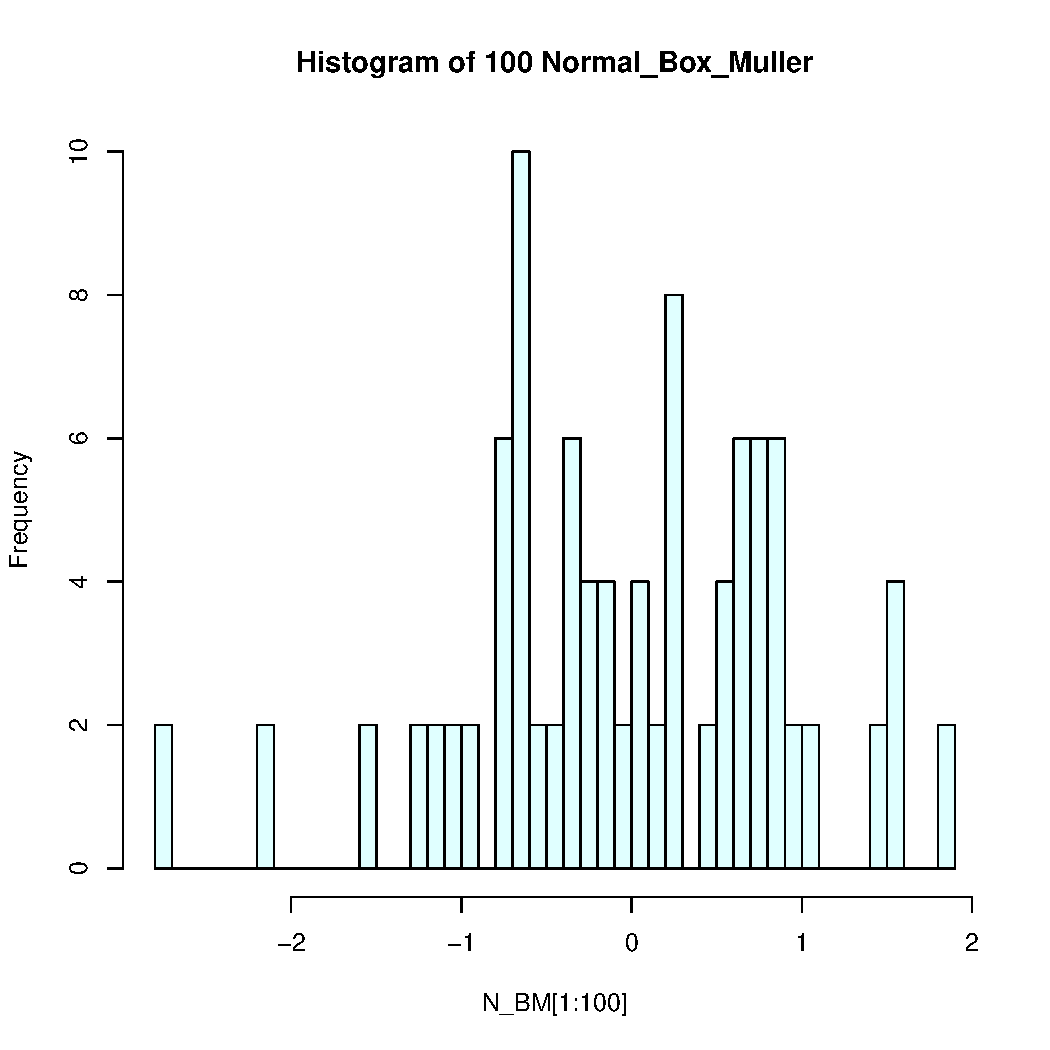
\includegraphics[width=0.45\textwidth]{N_BM100.pdf}}\hspace{10mm}
	\subfloat[500 samples]{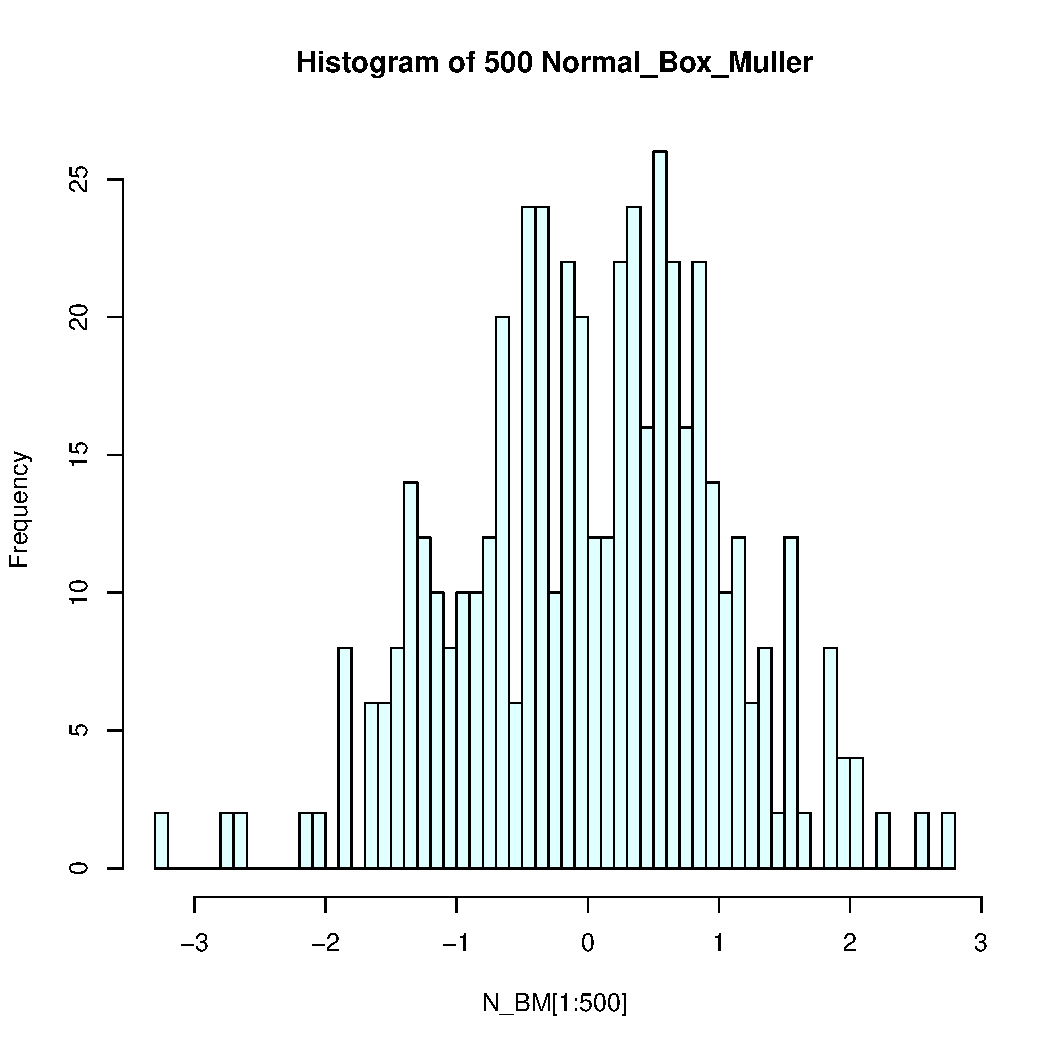
\includegraphics[width=0.45\textwidth]{N_BM500.pdf}}\\
	\subfloat[10000 samples]{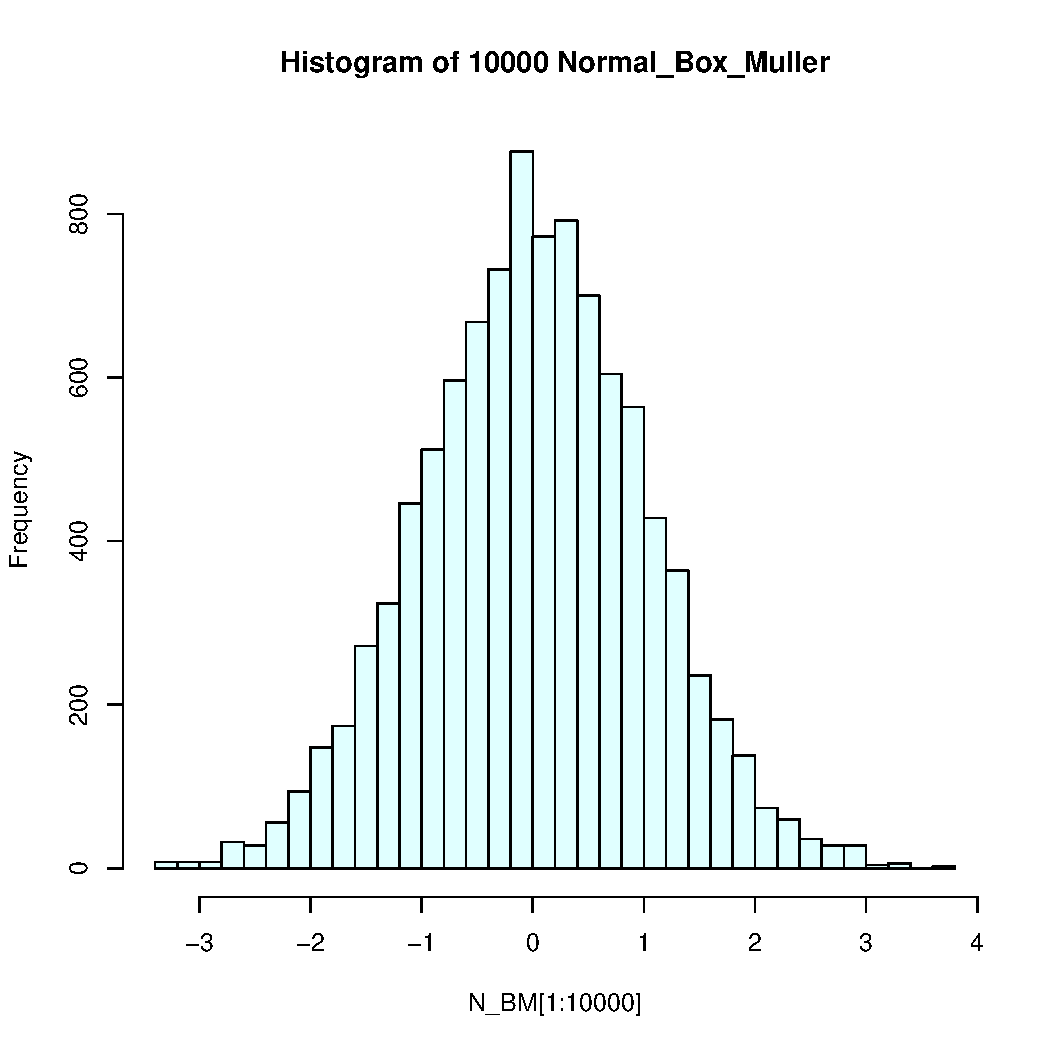
\includegraphics[width=0.45\textwidth]{N_BM10000.pdf}}
		\caption{Histogram for Box-Muller method}
\end{figure}

Using Box-Muller method, the sample mean, and the sample variance, for different values of sample size, are calculated to be:\\
Sample size = 100	\hspace{10mm}::\hspace{10mm}	Mean = -0.01703602	\hspace{8mm};\hspace{10mm}	Variance = 0.866979\\
Sample size = 500	\hspace{10mm}::\hspace{10mm}	Mean = 0.03307071	\hspace{10mm};\hspace{10mm}	Variance = 0.9975302\\
Sample size = 10000	\hspace{6mm}::\hspace{10mm}		Mean = 0.008148474	\hspace{8mm};\hspace{10mm}	Variance = 1.011222.\\
These values are close to the theoretical ones, 0, and 1.\\

\begin{figure}[H]
	\centering
	\subfloat[100 samples]{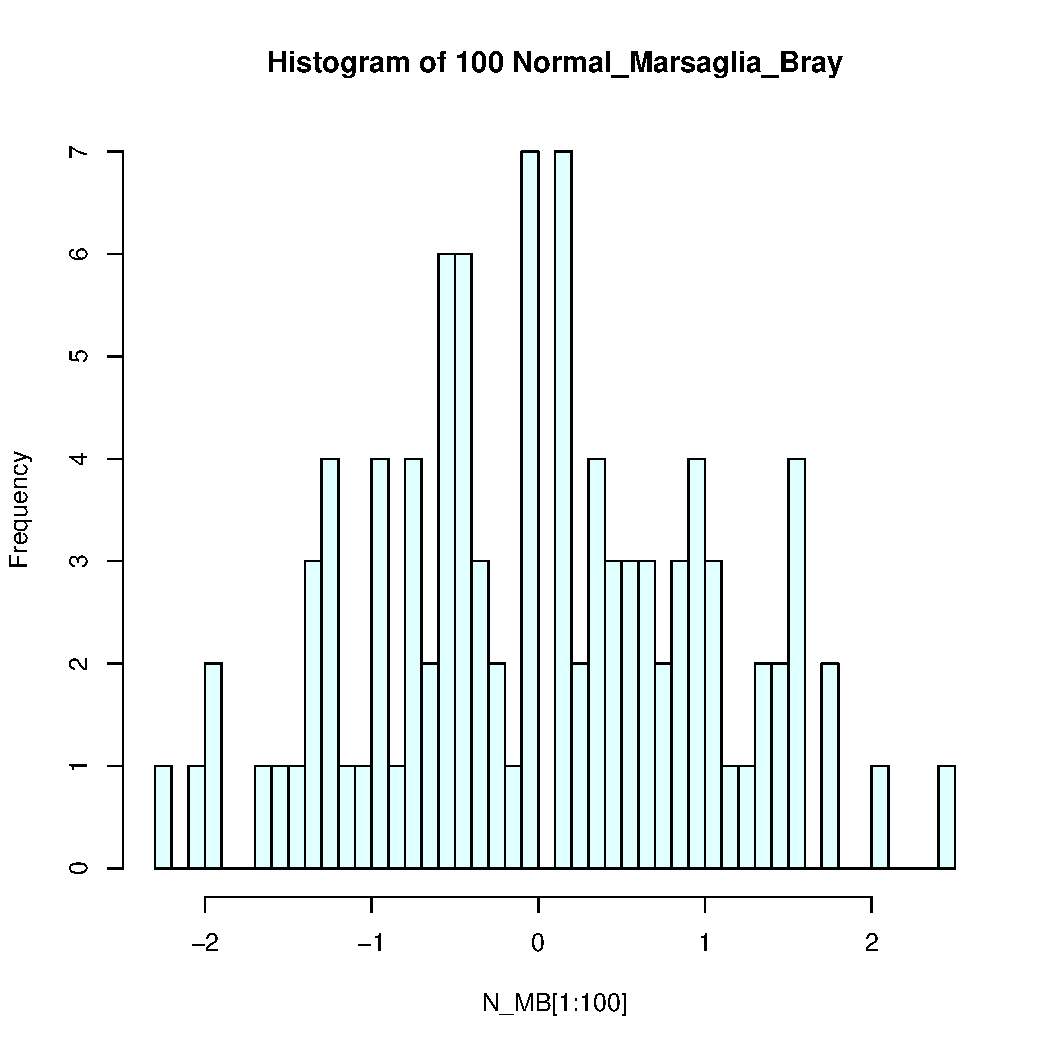
\includegraphics[width=0.45\textwidth]{N_MB100.pdf}}\hspace{10mm}
	\subfloat[500 samples]{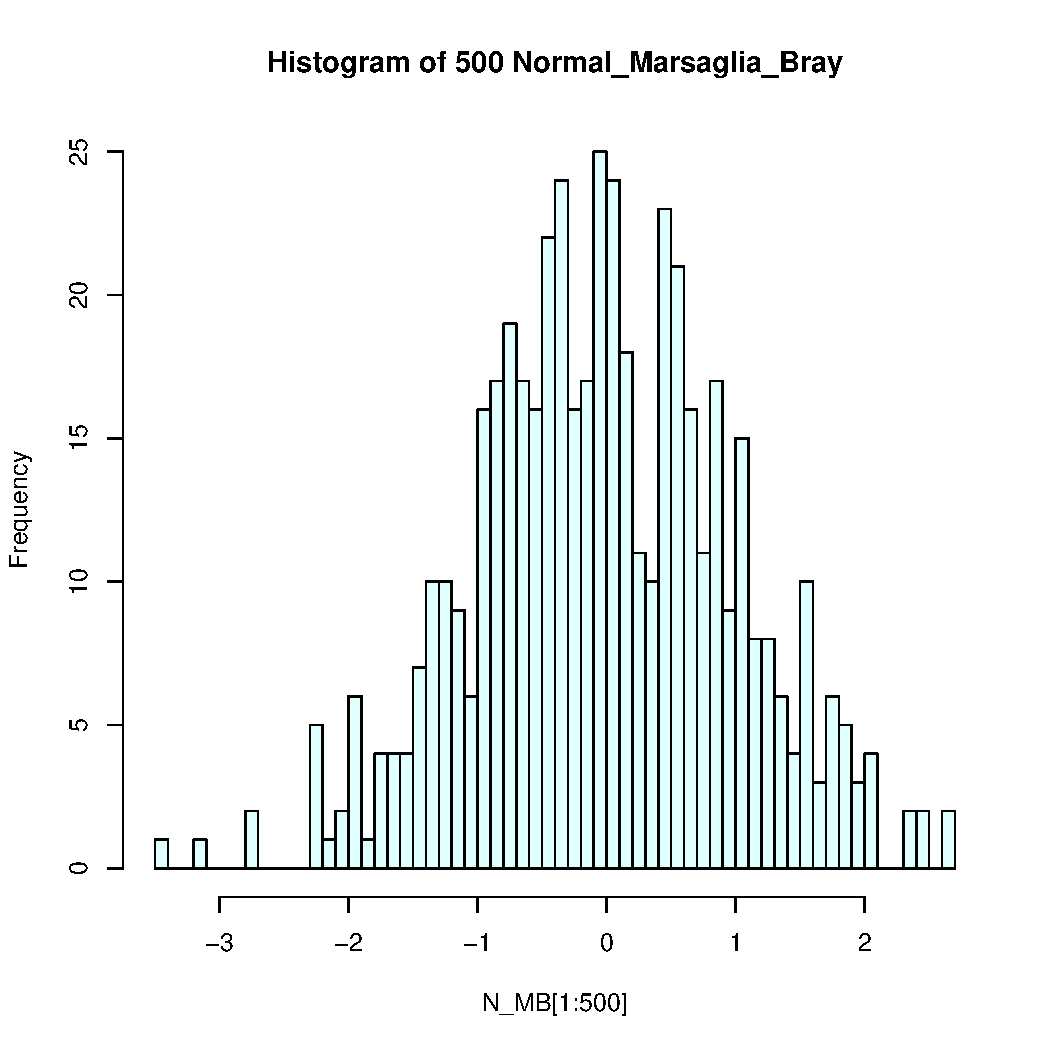
\includegraphics[width=0.45\textwidth]{N_MB500.pdf}}\\
	\subfloat[10000 samples]{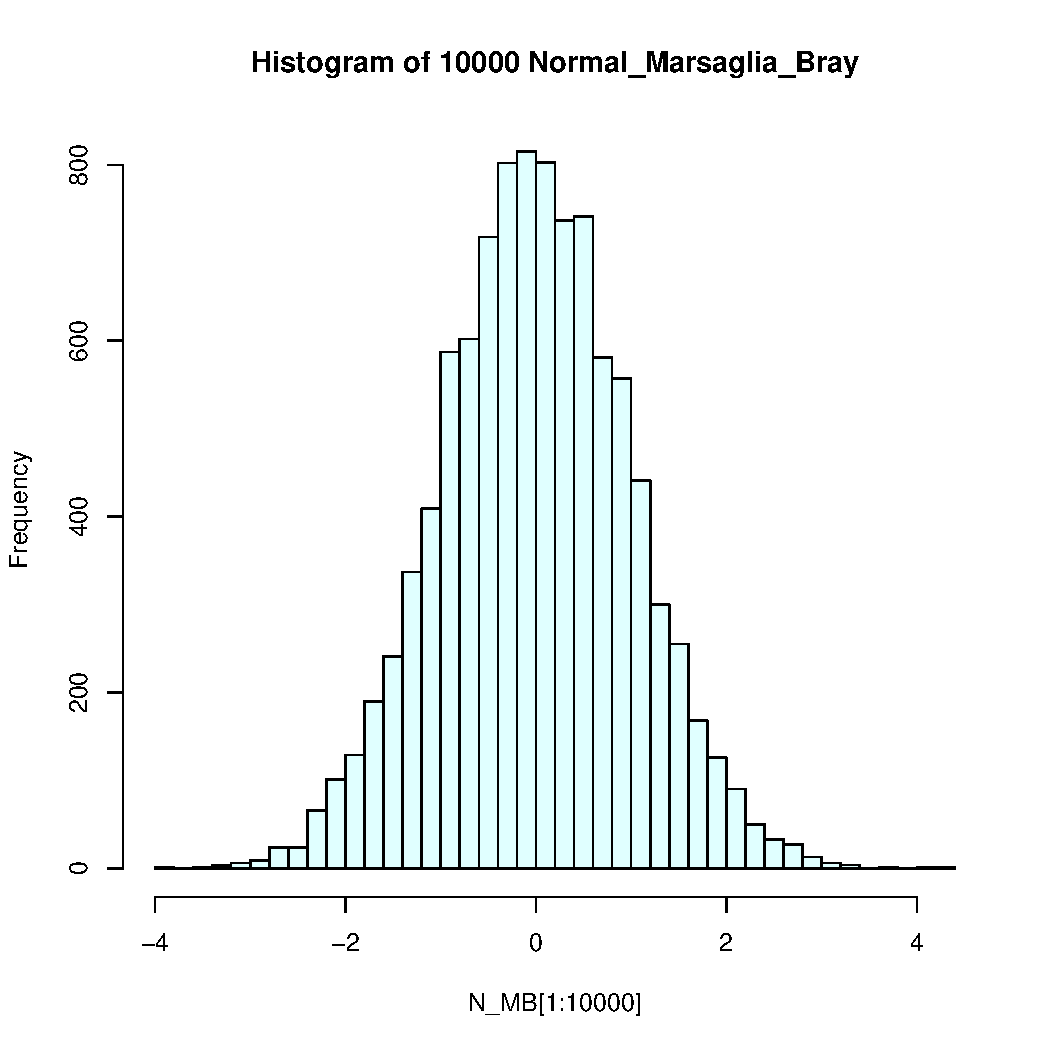
\includegraphics[width=0.45\textwidth]{N_MB10000.pdf}}
		\caption{Histogram for Marsaglia-Bray method}
\end{figure}

Using Marsaglia-Bray method, the sample mean, and the sample variance, for different values of sample size, are calculated to be:\\
Sample size = 100	\hspace{10mm}::\hspace{10mm}	Mean = -0.001358307	\hspace{8mm};\hspace{10mm}	Variance = 1.009955\\
Sample size = 500	\hspace{10mm}::\hspace{10mm}	Mean = -0.02857793	\hspace{10mm};\hspace{10mm}	Variance = 0.9973459\\
Sample size = 10000	\hspace{6mm}::\hspace{10mm}		Mean = -0.009924773	\hspace{8mm};\hspace{10mm}	Variance = 0.9804145.\\
These values are close to the theoretical ones, 0, and 1.\\

\begin{figure}[H]
	\centering
	\subfloat[$\mathcal{N}(0,5)$]{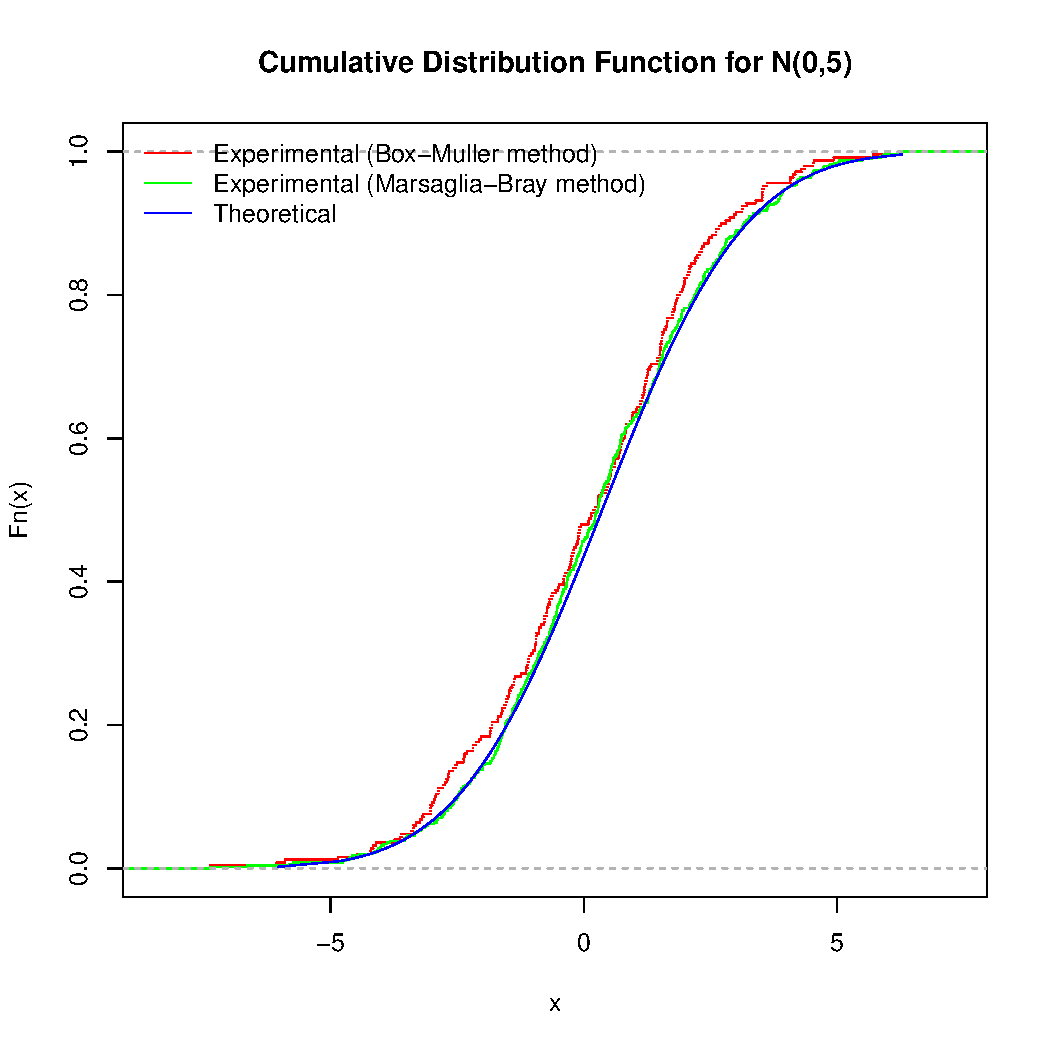
\includegraphics[width=0.65\textwidth]{N(0,5).pdf}}\\
	\subfloat[$\mathcal{N}(5,5)$]{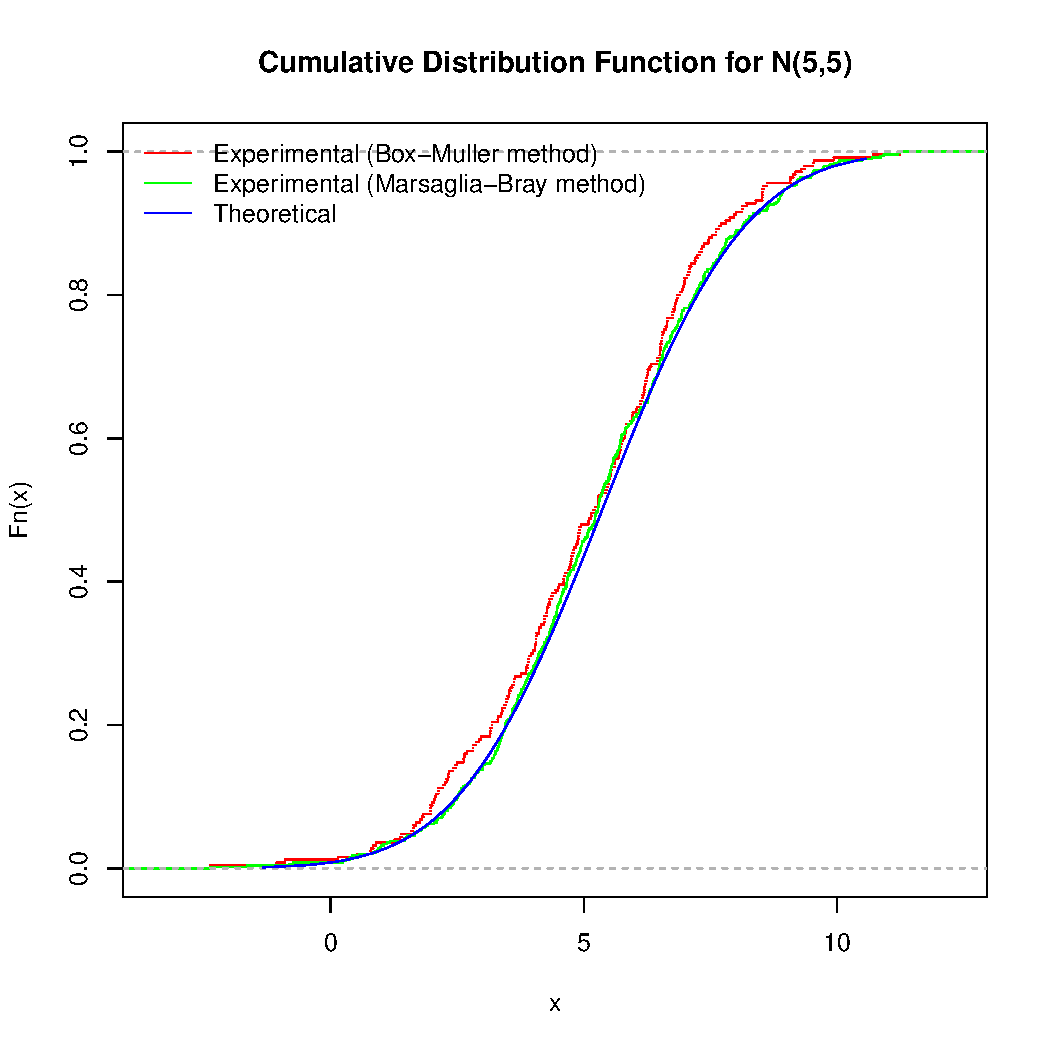
\includegraphics[width=0.65\textwidth]{N(5,5).pdf}}
		\caption{Plot of Cumulative Distribution Function}
\end{figure}

Computional time (elapsed time) for Box-Muller method and Marsaglia-Bray method are  0.041 , and  0.04 respectively.
Marsaglia-Bray method is faster than Box-Muller method.

For the Marsaglia-Bray method the proportion of values rejected (in generating 10000 sample values) is  0.2181392.\\
The value is close to theoretical one, $1-\frac{\pi}{4} = 0.2146018$.
\end{document}

%#Made by Ayush Sharma#
%#Signed as AShar#